\section{Ablation Studies}
\label{sec:ablations}
\paragraph{Overview.}
We vary the Critic architecture and intervention trigger, changing one component at a time while keeping the rest at the default configuration. All variants use the same three RoboCasa analysis tasks and $2H_{\mathrm{ref}}$ budgets as the Critic training-data experiment in Section~\ref{sec:main_results} and the retraction experiment in \cref{sec:data-retraction}.

\begin{table}[!t]
\centering
\small
\caption{Critic architecture. The MLP and KAN read only the latest query; the GRU and Transformer read the last eight. Success rate (\%), averaged over three tasks.}
\label{tab:critic-arch}
\begin{tabular}{@{}lccc@{}}
\toprule
Critic & Params & Q AUROC & Success \\
\midrule
\rowcolor{linkblue!12}
GRU (ours)  & 0.44M & 0.897 & 71.3 \\
MLP         & 0.35M & 0.886 & 71.1 \\
KAN         & 1.17M & 0.939 & 77.6 \\
Transformer & 0.62M & 0.915 & 73.6 \\
\bottomrule
\end{tabular}
\end{table}


\noindent\textbf{Critic Architecture.}
We also test whether ACRO depends on a particular Critic design. We replace the GRU with an MLP and a KAN that read only the latest query, and with a Transformer over the same eight-query window, all reading the same policy features. \Cref{tab:critic-arch} shows that every Critic improves over Base VLA and that success follows the Critic's AUROC. The MLP matches the GRU (71.1\% versus 71.3\%), the Transformer reaches 73.6\%, and the KAN attains both the highest AUROC (0.939) and the highest success (77.6\%), gaining 63 trials and losing 35 relative to the GRU. ACRO improves success with every tested architecture; across these fits, higher Critic AUROC is associated with higher task success.

\begin{figure}[!t]
\centering
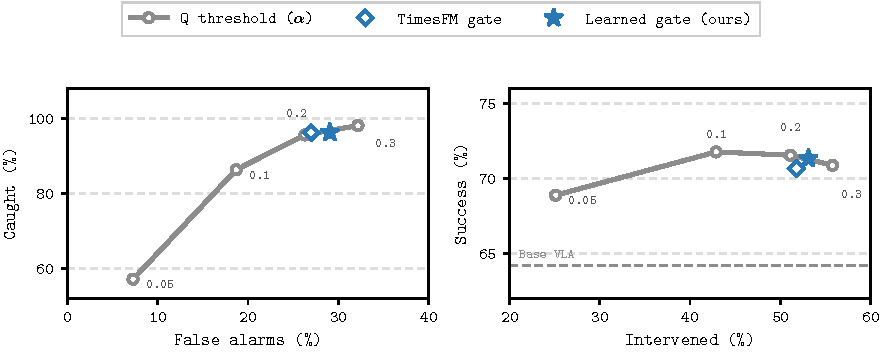
\includegraphics[width=\linewidth]{figures/trigger.pdf}
\caption{\textbf{Intervention trigger.} Gray points threshold Q at conformal level $\alpha$; both gates are calibrated at $\alpha=0.2$. Failures caught and false alarms are the fractions of executions that fail or succeed under Base VLA in which the trigger intervenes. Averaged over three tasks (450 paired trials).}
\label{fig:trigger}
\end{figure}


\noindent\textbf{Intervention Trigger.}
Finally, the trigger trades missed failures against unnecessary interruptions of executions that would have succeeded. We vary the conformal level $\alpha$ of a Q threshold and compare it with our learned gate on the recent Q history and with a gate that forecasts Q using TimesFM. \Cref{fig:trigger} plots the fraction of failures each trigger catches against its false-alarm rate, and success against how often it intervenes. The learned gate (96.3\% with 29.1\%) and the TimesFM gate (96.3\% with 27.0\%) fall on the same trade-off as the threshold at $\alpha=0.2$ (95.7\% with 26.3\%). Success saturates once most failures are caught: every trigger with $\alpha\ge0.1$ reaches 70.7\% to 71.8\%, whereas $\alpha=0.05$ reaches 68.9\%. Thus, on these tasks, how many failures the trigger catches matters more than whether it reads the level or the trend of Q.

\FloatBarrier
